\scanpage{44}
\diagram{\begin{array}{cccc}
&U&\subset V&\subset W\\
\deleted{\text{dim}}&&&\\
\text{dim:}&r&r+s&r+s+t
\end{array}}

$U$ \deleted{\unsure{est}} régulier

$V-U$ régulier

$W-V$ \deleted{\unsure{est}} régulier

$(V,W)$ \unsure{équisinguliers|équisingulier} le long de $\unsure{U}$

$W$ équisingulier le long de $V-U$

reconstruction

\deleted{$1^\circ$ \unsure{$U$} \unsure{espace}}

$1^\circ)$ $U$ espace régulier (dim $r$)

$2^\circ)$ $U'$ fibré sur $U$, fibres régulières (de dim $s-1$) donc $U'$ régulier

$3^\circ)$ $V^\circ$ variété à bord, de bord $U'$ (dim $r+s$)

$4^\circ)$ $V^{\circ\prime}$ fibré sur $V^\circ$, \deleted{des} fibres régulières (de dim $t-1$)

(sa dim est $r+s+t-1$), son bord est
\[
V^{\circ\prime}|\partial V^\circ=V^{\circ\prime}|U'
\]
(de dim $r+s+t-2$), fibré sur $U$: fibres régulières

$5^\circ)$ $U''$ autre fibré sur $U$ \inserted{(dim $r+s+t-1$)}, à fibres des \deleted{espaces réguliers} \inserted{variétés} à bord \inserted{(de dim $s+t-1$)} donc $\partial U''=$ fibré des bords (de dim $r+s+t-2$, fibres de dim $s+t-2$)

\margin{\diagram{\begin{tikzcd}[column sep=small,row sep=small]
&&V'=\partial W^\circ\unsure{\hookrightarrow|\subset} W^\circ\\
U''\arrow[dd]\arrow[urr,bend left=25]&\partial U''\arrow[l,hook]\arrow[d,equal]&\\
&\partial V^{\circ\prime}\arrow[r,hook]\arrow[d]&V^{\circ\prime}\arrow[uu,bend right=10]\arrow[d]\\
U&U'\arrow[l]\arrow[r,hook]\arrow[d,equal]&V^\circ\\
&\partial V^\circ&
\end{tikzcd}}
\figure{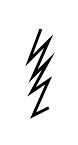
\begin{tikzpicture}[x=1cm,y=1cm]\draw[line width=1pt] (0,1.3)--(-.15,.9)--(.1,1.15)--(-.1,.7)--(.1,.9)--(-.12,.5)--(.1,.65)--(-.1,.2)--(.1,.3);\end{tikzpicture}}}

$6^\circ)$ Un isom. de $U$-fibrés en fibres régulières
\[
\partial U\unsure{=|\simeq}\partial V^{\prime\circ}
\]

On en conclut, par recollement, un \deleted{\unsure{variété sa}} espace régulier
\[
V'\deleted{\unsure{U}}=V^{\circ\prime}\amalg_{\partial V^{\circ\prime}=\partial U''}U''
\]

$7^\circ)$ \deleted{espace} \inserted{variété à bord} $W^\circ$, de bord $V'$

\figure{\begin{tikzpicture}[x=1cm,y=1cm]\draw (0,5.6)..controls(1.5,5.7)and(3,5.65)..(4.2,5.6)..controls(4.4,5.1)and(3.9,4.7)..(4.2,4.1)..controls(4.5,3.5)and(4.3,3.1)..(4.3,2.7)--(3.65,2.1)..controls(3.25,1.6)and(3.1,1)..(2.8,.8)..controls(1.4,.7)and(.3,.6)..(-.2,.4);\end{tikzpicture}}

On construit

\margin{\diagram{\begin{tikzcd}[column sep=small,row sep=small]
&&W^\circ\arrow[d,-{Hooks[harpoon]}]\\
&&V'=\partial W^\circ\\
\deleted{\unsure{U''}}\arrow[urr]&\deleted{\unsure{\partial U''}}\arrow[l,hook]&\\
U''\arrow[d]&\partial U''=\partial V^{\circ\prime}\arrow[l,hook]\arrow[r,hook]\arrow[d,"\text{cart}"']&V^{\circ\prime}\arrow[uu,hook]\arrow[d]\\
U&U'\arrow[l]\arrow[r,hook]\arrow[d,equal]&V^\circ\\
&(\partial V^\circ)&
\end{tikzcd}}}

$a)$ \deleted{\unsure{$U$}} $V=V^\circ\amalg_{U'}U$ et $U\hookrightarrow V$,
\diagram{\begin{tikzcd}[column sep=small,row sep=small]
&\unsure{V'|V''}\arrow[rrr]\arrow[d,equal]&&&V\arrow[d,equal]&\\
V^{\circ\prime}\arrow[rrr,bend right=40]&\amalg_{\partial}\arrow[rrr,bend right=55]&U''\arrow[rrr,bend right=35]&V^\circ&\amalg_{U'}&U
\end{tikzcd}}

\deleted{$b)\quad W=W^\circ\amalg$}

$b)$ $W=W^\circ\amalg_{V'}V$ et $V\longrightarrow W$
\mspage{45}
